\addcontentsline{toc}{subsection}{Imagens}
\subsection*{Imagens}

\begin{figure}[ht]
	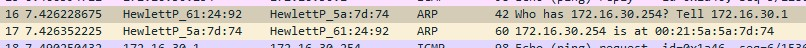
\includegraphics[width=\linewidth]{figure1}                                                      
    \caption{Pacotes ARP}
    \label{fig:fig1}
\end{figure}

\begin{figure}[ht]
	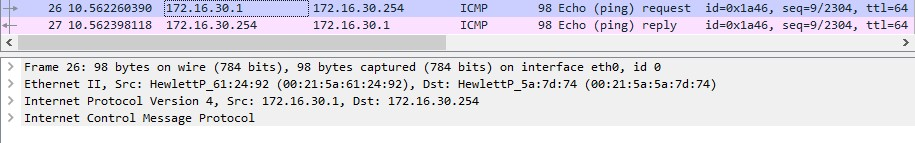
\includegraphics[width=\linewidth]{figure2}                                                      
    \caption{Pacote de Pedido}
    \label{fig:fig2}
\end{figure}

\begin{figure}[ht]
	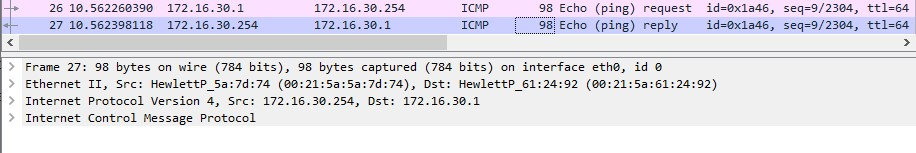
\includegraphics[width=\linewidth]{figure3}                                                      
    \caption{Pacote de Resposta}
    \label{fig:fig3}
\end{figure}

\begin{figure}[ht]
	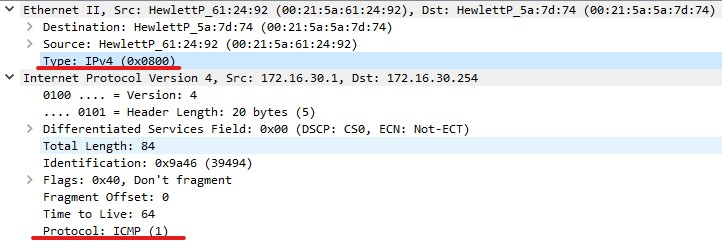
\includegraphics[width=\linewidth]{figure4}                                                      
    \caption{Campo Type Pacote ICMP}
    \label{fig:fig4}
\end{figure}

\begin{figure}[ht]
	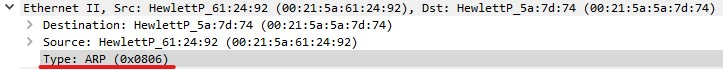
\includegraphics[width=\linewidth]{figure5}                                                      
    \caption{Campo Type Pacote ARP}
    \label{fig:fig5}
\end{figure}

\begin{figure}[ht]
	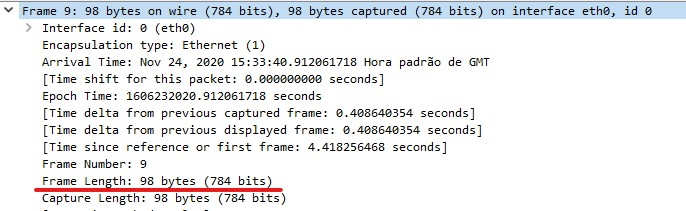
\includegraphics[width=\linewidth]{figure6}                                                      
    \caption{Tamanho de uma trama Recetora}
    \label{fig:fig6}
\end{figure}

\begin{figure}[ht]
	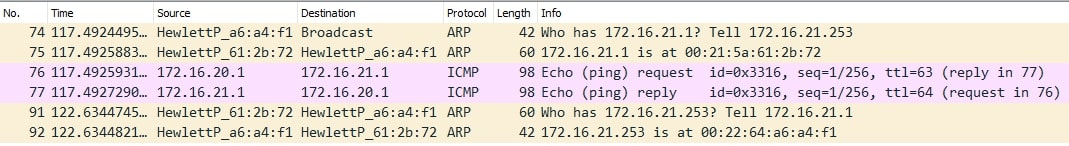
\includegraphics[width=\linewidth]{figure7}                                                      
    \caption{Pacotes ARP carta eth1 tux4}
    \label{fig:fig7}
\end{figure}

\begin{figure}[ht]
	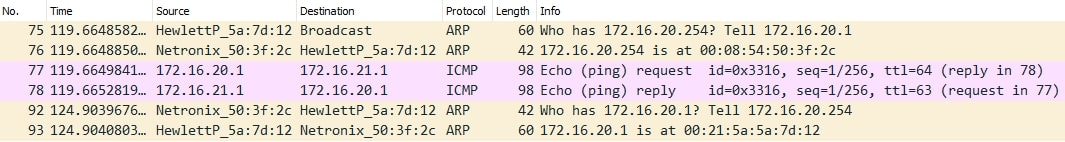
\includegraphics[width=\linewidth]{figure8}                                                      
    \caption{Pacotes ARP carta eth0 tux4}
    \label{fig:fig8}
\end{figure}

\begin{figure}[ht]
	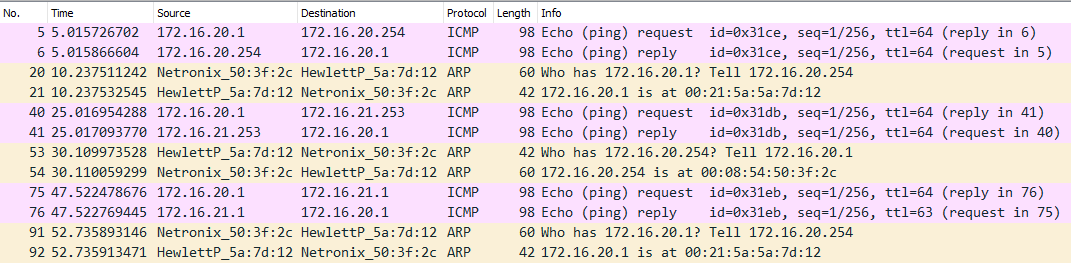
\includegraphics[width=\linewidth]{figure9}                                                      
    \caption{Pacotes ICMP com rotas definidas}
    \label{fig:fig9}
\end{figure}

\begin{figure}[ht]
	\begin{lstlisting}[language=bash]
	Cisco NAT
	http://www.cisco.com/en/US/tech/tk648/tk361/technologies_tech_note09186a0080094e77.shtml
	
	> conf t
	> interface gigabitethernet 0/0 *
	> ip address 172.16.y1.254 255.255.255.0
	> no shutdown
	> ip nat inside
	> exit
	
	> interface gigabitethernet 0/1*
	> ip address 172.16.1.y9 255.255.255.0
	> no shutdown
	> ip nat outside
	> exit
	
	> ip nat pool ovrld 172.16.1.y9 172.16.1.y9 prefix 24
	> ip nat inside source list 1 pool ovrld overload
	> access-list 1 permit 172.16.y0.0 0.0.0.7
	> access-list 1 permit 172.16.y1.0 0.0.0.7
	> ip route 0.0.0.0 0.0.0.0 172.16.1.254
	> ip route 172.16.y0.0 255.255.255.0 172.16.y1.253
	> end
	\end{lstlisting}
    \caption{Configuração NAT router}
    \label{fig:fig10}
\end{figure}

\begin{figure}[ht]
	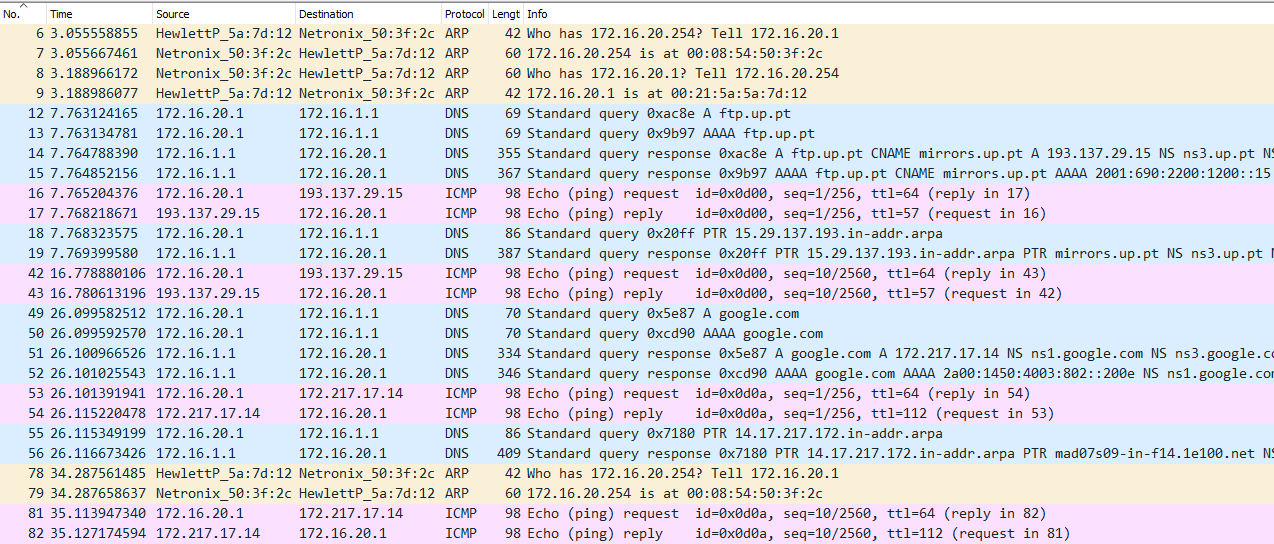
\includegraphics[width=\linewidth]{figure11}                                                      
    \caption{Pacotes DNS}
    \label{fig:fig11}
\end{figure}

\begin{figure}[ht]
	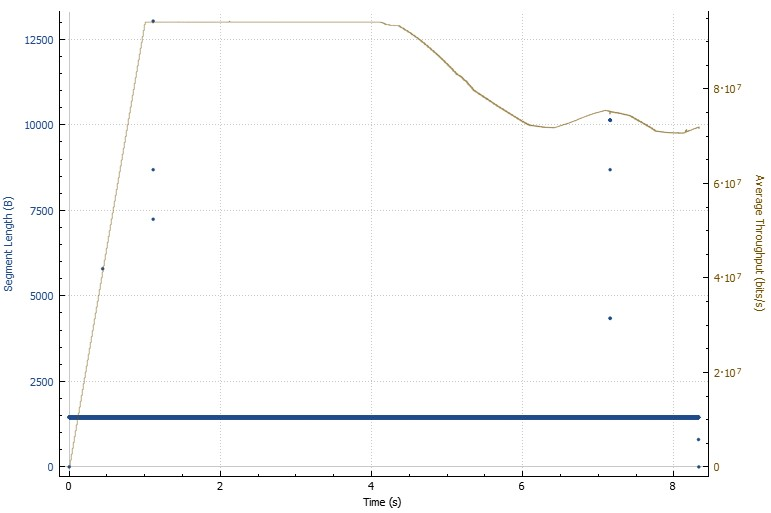
\includegraphics[width=\linewidth]{figure12}                                                      
    \caption{Throughtput TCP}
    \label{fig:fig12}
\end{figure}

